\documentclass[11pt]{article}
%this is for cyrillic text
\usepackage[main=russian,english]{babel}
%this is needed for changing font
\usepackage{fontspec}
\usepackage[a4paper, top=1cm]{geometry}
%without this double integral \iint doesnt work
\usepackage{mathtools}
\usepackage{physics}
%Чтобы LaTeX-овские лигатуры работали, типа тире, кавычек и прочего
\newfontfamily\cyrillicfont[Mapping=tex-text]{Times New Roman}
\usepackage{pgfplots}
\pgfplotsset{compat=1.8}
%this font has cyrillic letters
\setmainfont{Times New Roman}
\begin{document} 
\pagestyle{empty}
\textbf{4.}Вычислить поток векторного поля $\vec{a} = a_x(x,y,z)\vec{i} + a_y(x,y,z)\vec{j} + a_z(x,y,z)\vec{k}$ из тела $T$, ограниченного указанными поверхностями, двумя способами: с помощью поверхностного интеграла 1-го рода и с помощью поверхностного интеграла 2-го рода. Результат проверить с помощью Th Гаусса-Остроградского.\[T: z = -1 + \sqrt{x^2 + y^2}, z = 0, y = 0 (y \geq 0);\] \[\vec{a} = \vec{i} + 2y\vec{j}\]
Поверхностный интеграл 1-го рода:
\[\Pi = \iint_S a_ndS\]
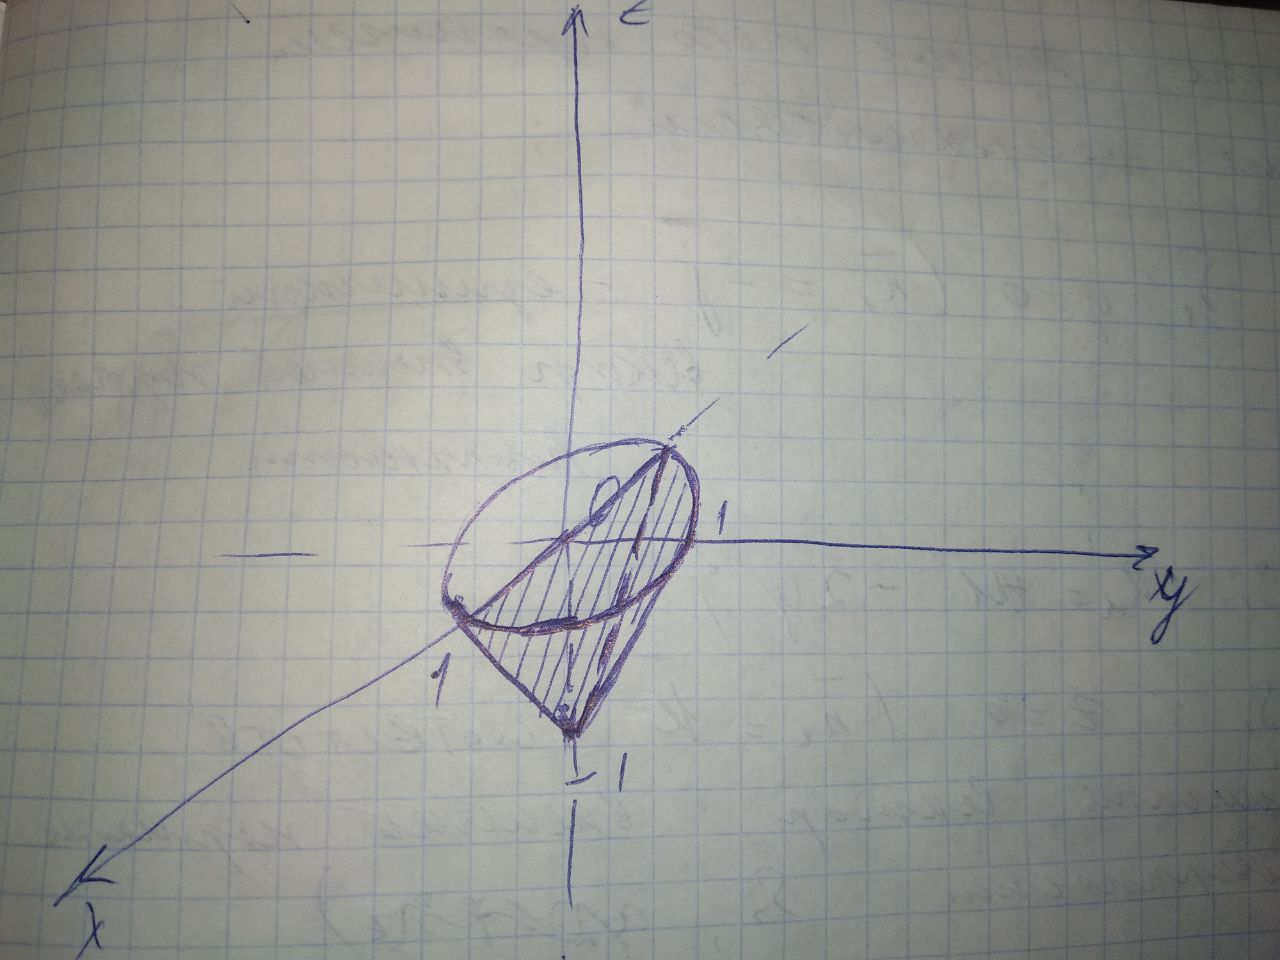
\includegraphics[scale=0.25]{xyz.jpg} 
\\
\textbf{Решение} (Поверхностный интеграл 1-го рода)
\\
Данное тело ограничено тремя поверхностями:
\[S1: y = 0 \quad (\vec{n}_1 = - \vec{j} \text{ - единичный вектор внешней нормали к поверхности $S_1$})\]
\[S_1: a_n = -2y;\]
\[S_2: z = 0 \quad (\vec{n}_2 = \vec{k} \text{ - соответств. единичный вектор внешней нормали к поверхности $S_2$)} \]
\[S_2: a_n = 0\]
$S_3$ - часть конуса $z = - 1 + \sqrt{x^2 + y^2}$.\\
Вычислим \[p(x,y) = \frac{1\cdot 1 \cdot 2x}{2\sqrt{x^2 + y^2}} = \frac{x}{\sqrt{x^2 + y^2}} = \frac{\partial z}{\partial x}\text{.}\]
\[q{x,y} = \frac{y}{\sqrt{x^2 + y^2}} = \frac{\partial z}{\partial y}\text{.}\]
\[dS = \sqrt{1 + p^2(x,y) + q^2(x,y)}dxdy = \sqrt{1 + \frac{x^2}{x^2 + y^2} + \frac{y^2}{x^2 + y^2}}dxdy = \sqrt{2}dxdy \]

Нормаль $\vec{n}_3$ образует тупой угол с осью $Oz$, т.е. соответствует нижней стороне поверхности $S_3$, следовательно,
\[cos\lambda = \frac{p(x,y)}{\sqrt{1 + p^2(x,y) + q^2(x,y)}} = \frac{x}{\sqrt{2}\cdot \sqrt{x^2 + y^2}}\]
\[cos\mu = \frac{q(x,y)}{\sqrt{1 + p^2(x,y) + q^2(x,y)}} = \frac{y}{\sqrt{2}\cdot \sqrt{x^2 + y^2}}\]
\[cos\nu = \frac{-1}{\sqrt{1 + p^2(x,y) + q^2(x,y)}} = - \frac{1}{\sqrt{2}}\]
\[a_n = \frac{x}{\sqrt{x^2 + y^2}} + \frac{2y^2}{\sqrt{x^2 + y^2}}\]
\[\Pi = \Pi_1 + \Pi_2 + \Pi_3\]
\[\Pi_1 = \iint_{S_1} a_ndS = \iint_{S_1} -2ydxdz = 0 \text{,}\]
т.к. на поверхности $S_1$ \quad $y = 0$
\[\Pi_2 = \iint_{S_2} a_{n_2}dS = 0 \text{,}\]
т.к. $a_{n_2} = 0$
\[\Pi_3 = \iint_{S_3}(a_xcos\lambda + a_ycos\mu + a_zcos\nu)dS = \]
\[= \iint_{S_3}\bigg(\frac{x}{\sqrt{2}\cdot \sqrt{x^2 + y^2}} + \frac{2y^2}{\sqrt{2}\cdot \sqrt{x^2 + y^2}}\bigg)dS = \]
\begin{center}
(поверхностный интеграл)
\end{center}
\[
\iint_{D}\bigg(\frac{x}{\sqrt{2}\cdot \sqrt{x^2 + y^2}} + \frac{2y^2}{\sqrt{2}\cdot \sqrt{x^2 + y^2}}\bigg)\sqrt{2}dxdy =
\]
\begin{center}
(двойной интеграл)
\end{center}
\[\iint_D \frac{(x + 2y^2)\cdot \sqrt{2}}{\sqrt{2}\sqrt{x^2 + y^2}}dxdy = \iint_D \frac{x + 2y^2}{\sqrt{x^2 + y^2}}\]
Перейдём к полярным координатам
\[x = rcos\varphi, \quad y = rsin\varphi, \quad |I(r,\varphi)| = r \]
Получим
\[\Pi_3 = \iint_D \frac{rcos\varphi + 2r^2sin^2\varphi}{r}\cdot rdrd\varphi = \iint_D(rcos\varphi + 2r^2sin^2\varphi)drd\varphi\]
\[\int_0^{\pi}d\varphi\int_0^1(rcos\varphi + 2 r^2sin^2\varphi)dr\]
\[I_{\text{внутр}} = \int_0^1(rcos\varphi + 2r^2sin^2\varphi)dr = (\frac{r^2}{2}cos\varphi + \frac{2r^3}{3}sin^2\varphi)\Bigg|_0^1 =\]
\[ = \frac{1}{2}cos\varphi + \frac{2}{3}sin^2\varphi\]
\[\Pi_3 = \int_0^{\pi}(\frac{1}{2}cos\varphi + \frac{2}{3}sin^2\varphi)d\varphi = \frac{1}{2}sin\varphi\Bigg|_0^{\pi} + I_2;\]
\[I_2 = \int_0^{\pi} \frac{2}{3}sin^2\varphi = \frac{2}{3}\int_0^\pi sin^2\varphi d\varphi = \]
\[ = \frac{2}{3}\int_0^\pi \frac{1}{2}(1 - cos2\varphi)d\varphi = \frac{2}{3}\int_0^\pi (\frac{1}{2} - \frac{1}{2}cos2\varphi)d\varphi = \]
\[ = \frac{2}{3}\int_0^\pi \frac{1}{2}d\varphi + \frac{2}{3}\int_0^\pi(-\frac{1}{2}cos2\varphi)d\varphi = \frac{2}{3}\cdot\frac{1}{2}\varphi\Big|_0^\pi - \frac{1}{3}\int_0^\pi cos2\varphi d\varphi = \]
\[ = \frac{\pi}{3} - \frac{1}{3}\int_0^\pi \frac{1}{2} cos2\varphi d(2\varphi) = \frac{\pi}{3} - \frac{1}{6}(sin2\varphi)\Big|_0^\pi = \frac{\pi}{3} - 0 = \frac{\pi}{3}. \]
\[\Pi_3 = \frac{1}{2}sin\pi + \frac{\pi}{3} = \frac{1}{2}\cdot 0 + \frac{\pi}{3} = \frac{\pi}{3}\]
\textbf{Ответ}: $\frac{\pi}{3}$.

\textbf{2 способ (поверхностный интеграл 2-го рода)}\\
\textbf{Решение}\\
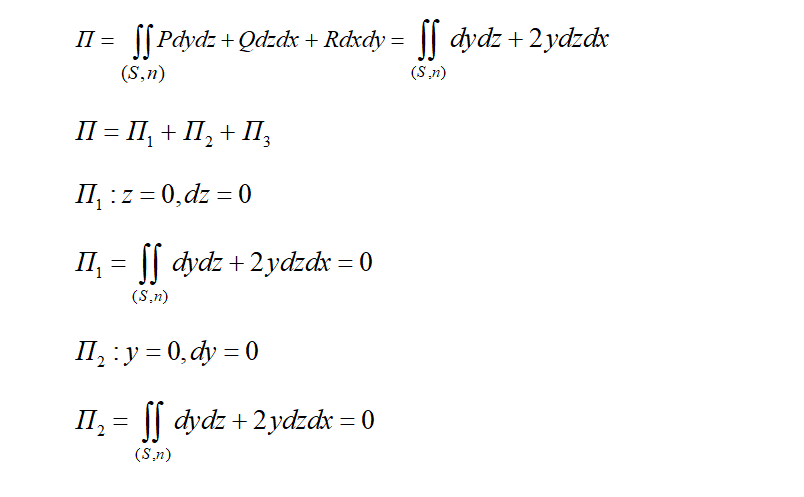
\includegraphics[scale=0.85]{screenshot.PNG} 
\\
Третья составляющая тела $T$ - поверхность 
\[S_3 (z = -1 + \sqrt{x^2 + y^2}) \]
Поток через неё:
\[\Pi_3 = \iint_{S_3}dydz + 2ydzdx = \iint_{D_{yz}}dydz + 2\iint_{D_{xz}}\sqrt{(z + 1)^2 - x^2}dzdx - \iint_{D_{yz}}dydz \]
Здесь 1ое и 3е слагаемые - это противоположеные по знаку значения, которые взаимоуничтожаются. Это вызвано тем, что поверхность $S_3$ симметрична относительно плоскости $zOy$. Проекция на эту плоскость состоит из двух частей. Перед интегралом по проекции части поверхности, лежащей в восьмом октанте берётся знак "+" т.к. угол между нормалью к поверхности и осью $Ox$ в этом случае острый. Перед интегралом по проекции части поверхности, лежащей в пятом октанте, берётся знак минус, т.к. угол между вектором нормали к этой части поверхности, направленным изнутри наружу, и осью $Ox$ тупой. Таким образом, после сокращения этих двух слагаемых, имеем
\[\Pi_3 = 2\iint_{D_{xz}}\sqrt{(z + 1)^2 - x^2}dzdx = \]
\begin{center}
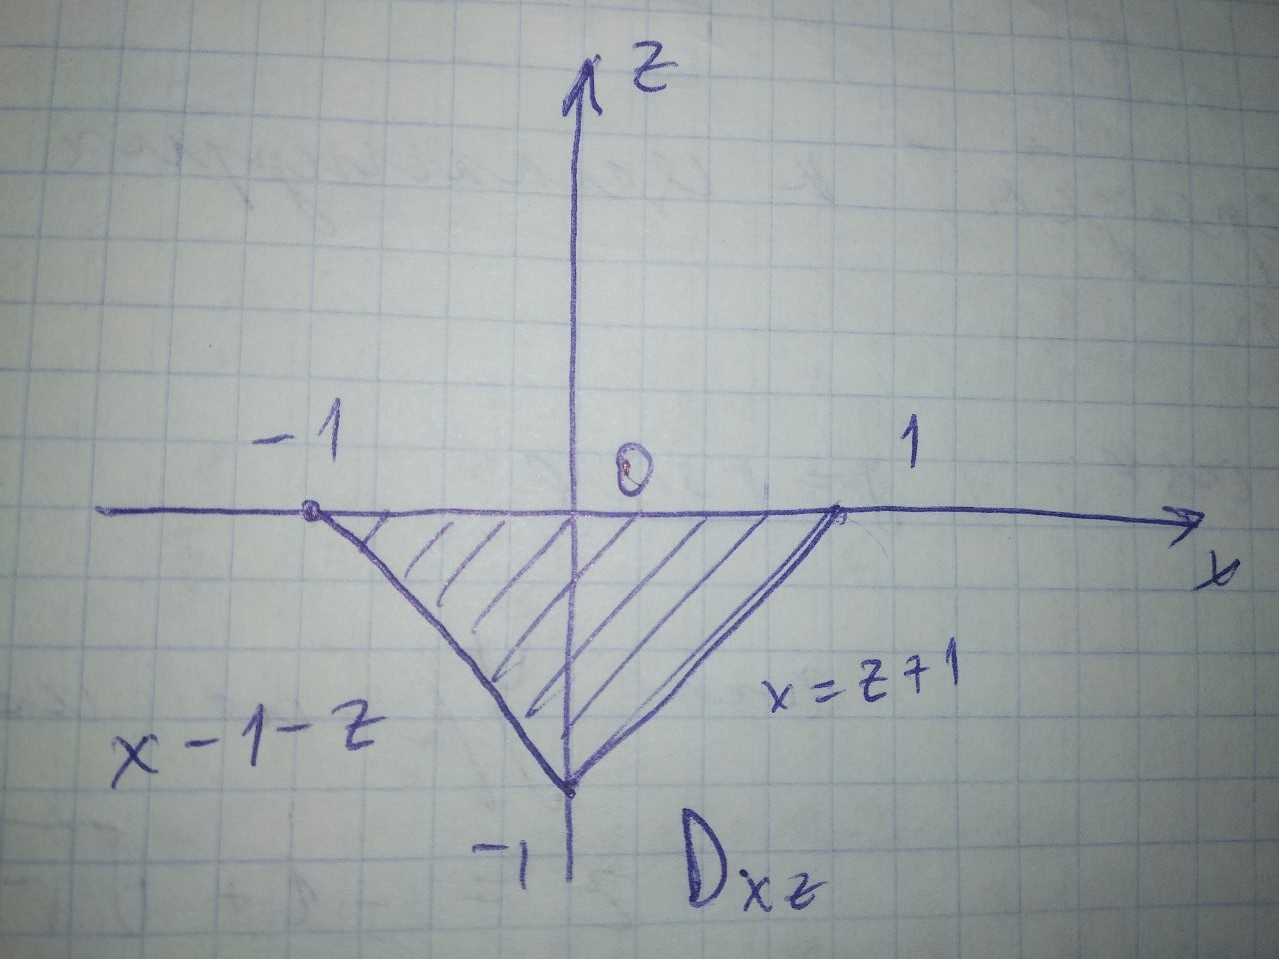
\includegraphics[scale=0.2]{4.jpg} 
\end{center}

\[2\int_{-1}^0dz\int_{-1-z}^{z+1}\sqrt{(z + 1)^2 - x^2}dx =\] \[= 2\int_{-1}^0dz\Big(\frac{x}{2}\cdot \sqrt{(z + 1)^2 - x^2} + \frac{(z + 1)^2}{2}arcsin\big(\frac{x}{z+1}\big)\Big)\Big|_{-1-z}^{z + 1} = \]
\[2\int_{-1}^0dz\Big(\frac{(z+1)^2}{2}\cdot \frac{\pi}{2} - \frac{(z + 1)^2}{2}\cdot (-\frac{\pi}{2})\Big) = \]
\[ = 2\int_{-1}^0\frac{2(z + 1)^2\cdot \pi}{4}dz = \pi \int_{-1}^0(z + 1)^2dz = \pi\int_{-1}^0(z^2 + 2z + 1)dz = \]
\[= \pi\eval{(\frac{z^3}{3} + z^2 + z)}_{-1}^0 = \pi(-(-\frac{1}{3} + 1 - 1)) = \frac{\pi}{3}\]
\[\Pi = \Pi_1 + \Pi_2 + \Pi_3 = 0 + 0 + \frac{\pi}{3} = \frac{\pi}{3}\]
\textbf{Ответ}: $\frac{\pi}{3}$
\\
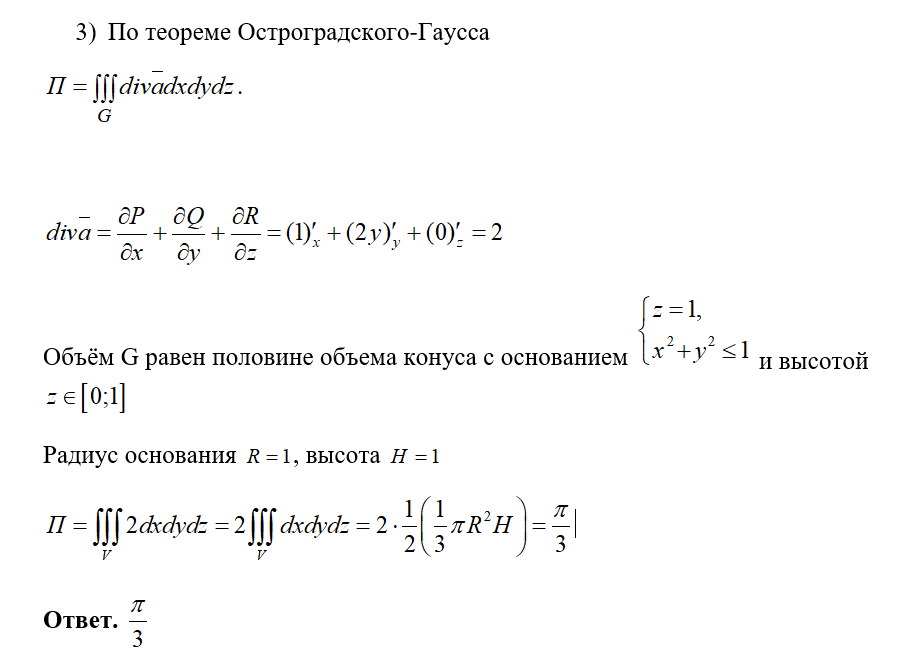
\includegraphics[scale=1]{screenshot1.PNG} 
\end{document}

